% Options for packages loaded elsewhere
\PassOptionsToPackage{unicode}{hyperref}
\PassOptionsToPackage{hyphens}{url}
%
\documentclass[
]{article}
\author{}
\date{\vspace{-2.5em}}

\usepackage{amsmath,amssymb}
\usepackage{lmodern}
\usepackage{iftex}
\ifPDFTeX
  \usepackage[T1]{fontenc}
  \usepackage[utf8]{inputenc}
  \usepackage{textcomp} % provide euro and other symbols
\else % if luatex or xetex
  \usepackage{unicode-math}
  \defaultfontfeatures{Scale=MatchLowercase}
  \defaultfontfeatures[\rmfamily]{Ligatures=TeX,Scale=1}
\fi
% Use upquote if available, for straight quotes in verbatim environments
\IfFileExists{upquote.sty}{\usepackage{upquote}}{}
\IfFileExists{microtype.sty}{% use microtype if available
  \usepackage[]{microtype}
  \UseMicrotypeSet[protrusion]{basicmath} % disable protrusion for tt fonts
}{}
\makeatletter
\@ifundefined{KOMAClassName}{% if non-KOMA class
  \IfFileExists{parskip.sty}{%
    \usepackage{parskip}
  }{% else
    \setlength{\parindent}{0pt}
    \setlength{\parskip}{6pt plus 2pt minus 1pt}}
}{% if KOMA class
  \KOMAoptions{parskip=half}}
\makeatother
\usepackage{xcolor}
\IfFileExists{xurl.sty}{\usepackage{xurl}}{} % add URL line breaks if available
\IfFileExists{bookmark.sty}{\usepackage{bookmark}}{\usepackage{hyperref}}
\hypersetup{
  hidelinks,
  pdfcreator={LaTeX via pandoc}}
\urlstyle{same} % disable monospaced font for URLs
\usepackage[margin=1in]{geometry}
\usepackage{color}
\usepackage{fancyvrb}
\newcommand{\VerbBar}{|}
\newcommand{\VERB}{\Verb[commandchars=\\\{\}]}
\DefineVerbatimEnvironment{Highlighting}{Verbatim}{commandchars=\\\{\}}
% Add ',fontsize=\small' for more characters per line
\usepackage{framed}
\definecolor{shadecolor}{RGB}{248,248,248}
\newenvironment{Shaded}{\begin{snugshade}}{\end{snugshade}}
\newcommand{\AlertTok}[1]{\textcolor[rgb]{0.94,0.16,0.16}{#1}}
\newcommand{\AnnotationTok}[1]{\textcolor[rgb]{0.56,0.35,0.01}{\textbf{\textit{#1}}}}
\newcommand{\AttributeTok}[1]{\textcolor[rgb]{0.77,0.63,0.00}{#1}}
\newcommand{\BaseNTok}[1]{\textcolor[rgb]{0.00,0.00,0.81}{#1}}
\newcommand{\BuiltInTok}[1]{#1}
\newcommand{\CharTok}[1]{\textcolor[rgb]{0.31,0.60,0.02}{#1}}
\newcommand{\CommentTok}[1]{\textcolor[rgb]{0.56,0.35,0.01}{\textit{#1}}}
\newcommand{\CommentVarTok}[1]{\textcolor[rgb]{0.56,0.35,0.01}{\textbf{\textit{#1}}}}
\newcommand{\ConstantTok}[1]{\textcolor[rgb]{0.00,0.00,0.00}{#1}}
\newcommand{\ControlFlowTok}[1]{\textcolor[rgb]{0.13,0.29,0.53}{\textbf{#1}}}
\newcommand{\DataTypeTok}[1]{\textcolor[rgb]{0.13,0.29,0.53}{#1}}
\newcommand{\DecValTok}[1]{\textcolor[rgb]{0.00,0.00,0.81}{#1}}
\newcommand{\DocumentationTok}[1]{\textcolor[rgb]{0.56,0.35,0.01}{\textbf{\textit{#1}}}}
\newcommand{\ErrorTok}[1]{\textcolor[rgb]{0.64,0.00,0.00}{\textbf{#1}}}
\newcommand{\ExtensionTok}[1]{#1}
\newcommand{\FloatTok}[1]{\textcolor[rgb]{0.00,0.00,0.81}{#1}}
\newcommand{\FunctionTok}[1]{\textcolor[rgb]{0.00,0.00,0.00}{#1}}
\newcommand{\ImportTok}[1]{#1}
\newcommand{\InformationTok}[1]{\textcolor[rgb]{0.56,0.35,0.01}{\textbf{\textit{#1}}}}
\newcommand{\KeywordTok}[1]{\textcolor[rgb]{0.13,0.29,0.53}{\textbf{#1}}}
\newcommand{\NormalTok}[1]{#1}
\newcommand{\OperatorTok}[1]{\textcolor[rgb]{0.81,0.36,0.00}{\textbf{#1}}}
\newcommand{\OtherTok}[1]{\textcolor[rgb]{0.56,0.35,0.01}{#1}}
\newcommand{\PreprocessorTok}[1]{\textcolor[rgb]{0.56,0.35,0.01}{\textit{#1}}}
\newcommand{\RegionMarkerTok}[1]{#1}
\newcommand{\SpecialCharTok}[1]{\textcolor[rgb]{0.00,0.00,0.00}{#1}}
\newcommand{\SpecialStringTok}[1]{\textcolor[rgb]{0.31,0.60,0.02}{#1}}
\newcommand{\StringTok}[1]{\textcolor[rgb]{0.31,0.60,0.02}{#1}}
\newcommand{\VariableTok}[1]{\textcolor[rgb]{0.00,0.00,0.00}{#1}}
\newcommand{\VerbatimStringTok}[1]{\textcolor[rgb]{0.31,0.60,0.02}{#1}}
\newcommand{\WarningTok}[1]{\textcolor[rgb]{0.56,0.35,0.01}{\textbf{\textit{#1}}}}
\usepackage{longtable,booktabs,array}
\usepackage{calc} % for calculating minipage widths
% Correct order of tables after \paragraph or \subparagraph
\usepackage{etoolbox}
\makeatletter
\patchcmd\longtable{\par}{\if@noskipsec\mbox{}\fi\par}{}{}
\makeatother
% Allow footnotes in longtable head/foot
\IfFileExists{footnotehyper.sty}{\usepackage{footnotehyper}}{\usepackage{footnote}}
\makesavenoteenv{longtable}
\usepackage{graphicx}
\makeatletter
\def\maxwidth{\ifdim\Gin@nat@width>\linewidth\linewidth\else\Gin@nat@width\fi}
\def\maxheight{\ifdim\Gin@nat@height>\textheight\textheight\else\Gin@nat@height\fi}
\makeatother
% Scale images if necessary, so that they will not overflow the page
% margins by default, and it is still possible to overwrite the defaults
% using explicit options in \includegraphics[width, height, ...]{}
\setkeys{Gin}{width=\maxwidth,height=\maxheight,keepaspectratio}
% Set default figure placement to htbp
\makeatletter
\def\fps@figure{htbp}
\makeatother
\setlength{\emergencystretch}{3em} % prevent overfull lines
\providecommand{\tightlist}{%
  \setlength{\itemsep}{0pt}\setlength{\parskip}{0pt}}
\setcounter{secnumdepth}{5}
\usepackage{booktabs}
\ifLuaTeX
  \usepackage{selnolig}  % disable illegal ligatures
\fi
\usepackage[]{natbib}
\bibliographystyle{plainnat}

\begin{document}

{
\setcounter{tocdepth}{2}
\tableofcontents
}
\hypertarget{introducciuxf3n}{%
\section{Introducción}\label{introducciuxf3n}}

La composición y estructura de la comunidad varía a lo largo de un gradiente ambiental o a lo largo del tiempo. De esta manera, si un ecólogo realiza un muestreo de ese gradiente, tendrá cambios en la composición de la comunidad (las especies que la constituyen) y en la estructura (las abundancias de las especies) (figura \ref{fig:com}).

\begin{figure}
\centering
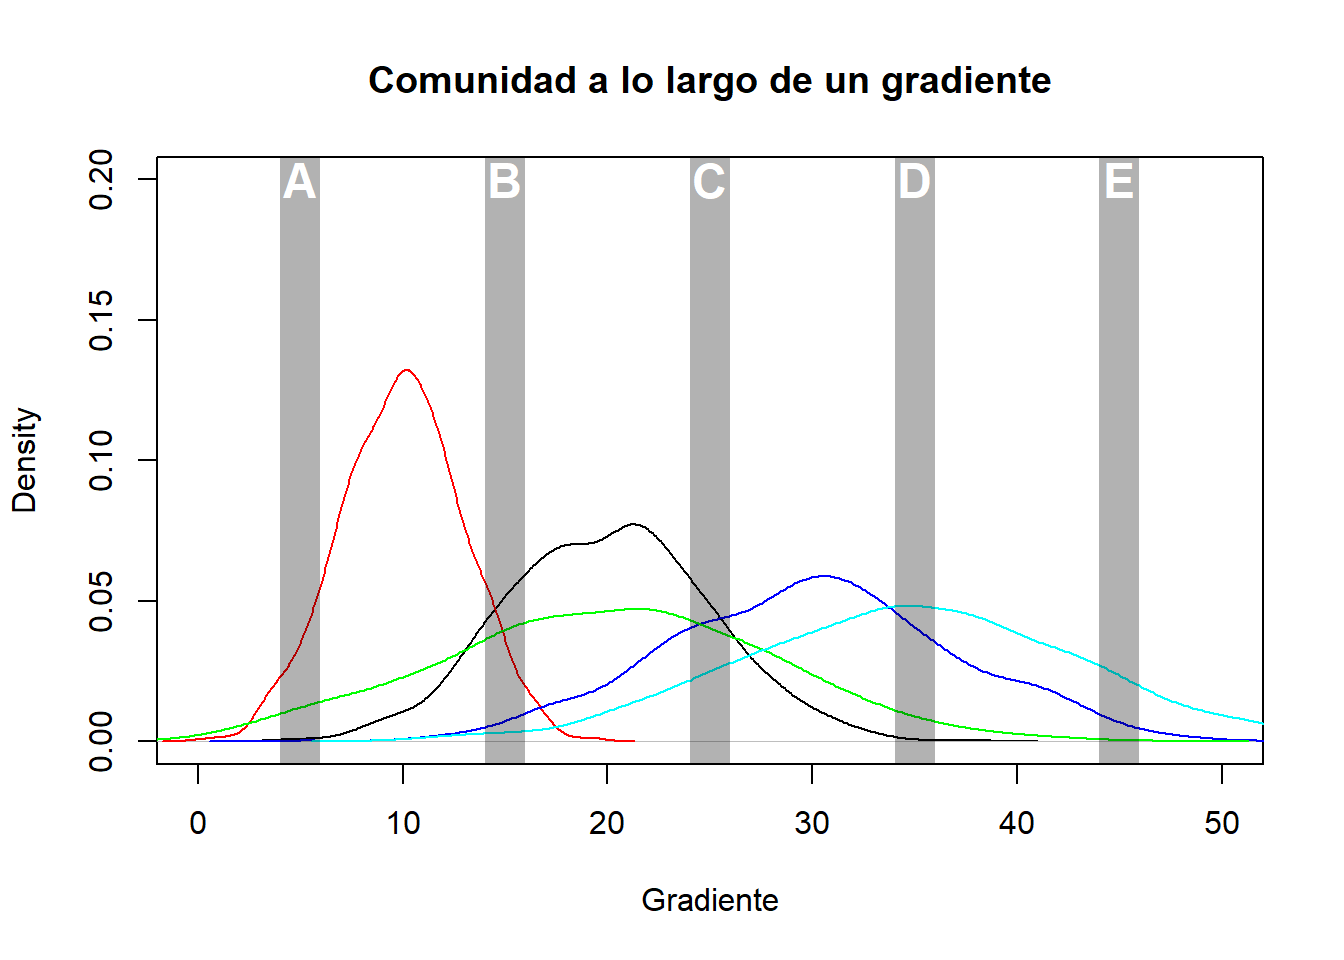
\includegraphics{02-Similitud_files/figure-latex/com-1.pdf}
\caption{\label{fig:com}Ejemplo de la variación de una comunidad}
\end{figure}

Como podemos ver en la figura \ref{fig:com}, en cada uno de los transectos (representados por la línea gris), la ocurrencia de las especies y su abundancia cambia. Por ejemplo, en el transecto ``B'' la comunidad está representada por cinco especies, la especie representada por la línea verde alcanza su máxima abundancia, mientras que la representada por la línea azul se encuentra con una abundancia muy baja. En la comunidad ``C'' tenemos cuatro especies pero las abundancias son diferentes a las encontradas en la comunidad ``B''. En el caso de la comunidad ``C'', no solo las abundancias varían sino también la ocurrencia de especies.

Los cambios en la estructura y composición de la comunidad hacen que ciertos transectos sean más parecidos entre sí que otros, en el caso del ejemplo las similitudes en cuanto a estructura y composición de las especies son más o menos claras, sin embargo, en la realidad es más complejo determinar a simple vista estas similitudes. A continuación, veremos los métodos que se usan para cuantificar estas similitudes.

\begin{center}\rule{0.5\linewidth}{0.5pt}\end{center}

\hypertarget{similitud-disimilitud-y-distancia}{%
\section{Similitud, disimilitud y distancia}\label{similitud-disimilitud-y-distancia}}

Dos elementos se parecen más cuando sus propiedades son más parecidas. Por ejemplo, si existen dos bosques dominados por Eucalyptus estos serán más parecidos entre ellos que con un bosque donde el guayacán sea dominante. Es decir, dos comunidades se parecerán más si su composición y estructura es similar. El cálculo de \emph{similitud} nos permite cuantificar en qué medida dos comunidades se parecen. Aunque esta información es interesante, cuando se analizan muchas comunidades, el apreciar estas diferencias entre cada par sería complejo, por lo que interesa representar estas comunidades en un plano. La graficación de las comunidades en un plano es posible si disponemos de medidas de \textbf{distancias} entre las comunidades. Las distancias es una medida de cuan diferentes son las comunidades entre sí y pueden ser estimadas a través de diferentes medidas como; distancias simétricas (ejemplo Euclideana, Hellinger), o a través de medidas asimétricas (medidas de \textbf{disimilitud}, la otra cara de la similitud).

\hypertarget{uxedndices-de-similitud}{%
\section{Índices de Similitud}\label{uxedndices-de-similitud}}

¿Cuán similares son dos localidades?, vamos a calcular dos tipos de similitudes una basada en incidencia (presencia-ausencia de especies) (ej. Índices de \emph{Sorensen}, \emph{Jaccard} y \emph{Simpson}), y otra basada en la abundancia, \emph{Porcentaje de Similitud}. Imaginemos que tenemos cuatro localidades (A, B, C, D) donde recogemos los datos de densidad de cuatro especies; \emph{Tabebuia billbergii}, \emph{Geoffroea spinosa},\emph{Ceiba trichistandra} y \emph{Colicodendron scabridum}, especies características de bosques secos tropicales. Podemos introducir datos hipotéticos de abundancia para cada especie en cada una de las localidades.

\begin{Shaded}
\begin{Highlighting}[]
\NormalTok{dens }\OtherTok{\textless{}{-}} \FunctionTok{data.frame}\NormalTok{(}\AttributeTok{T.bil =} \FunctionTok{c}\NormalTok{(}\DecValTok{1}\NormalTok{, }\DecValTok{1}\NormalTok{, }\DecValTok{2}\NormalTok{, }\DecValTok{3}\NormalTok{), }\AttributeTok{G.spi =} \FunctionTok{c}\NormalTok{(}\DecValTok{21}\NormalTok{, }\DecValTok{8}\NormalTok{, }\DecValTok{13}\NormalTok{, }\DecValTok{5}\NormalTok{),}
                   \AttributeTok{C.tri =} \FunctionTok{c}\NormalTok{(}\DecValTok{11}\NormalTok{, }\DecValTok{3}\NormalTok{, }\DecValTok{7}\NormalTok{, }\DecValTok{5}\NormalTok{), }\AttributeTok{C.sca =} \FunctionTok{c}\NormalTok{(}\DecValTok{16}\NormalTok{, }\DecValTok{0}\NormalTok{, }\DecValTok{9}\NormalTok{, }\DecValTok{4}\NormalTok{))}
\FunctionTok{row.names}\NormalTok{(dens) }\OtherTok{\textless{}{-}}\NormalTok{ LETTERS[}\DecValTok{1}\SpecialCharTok{:}\DecValTok{4}\NormalTok{]}
\NormalTok{dens}
\end{Highlighting}
\end{Shaded}

\begin{verbatim}
##   T.bil G.spi C.tri C.sca
## A     1    21    11    16
## B     1     8     3     0
## C     2    13     7     9
## D     3     5     5     4
\end{verbatim}

Generamos un gráfico basado en las dos primeras especies para ver cuánto se parece cada sitio (Figura \ref{fig:NMDS}).

\begin{Shaded}
\begin{Highlighting}[]
\FunctionTok{par}\NormalTok{(}\AttributeTok{mar=}\FunctionTok{c}\NormalTok{(}\DecValTok{4}\NormalTok{,}\DecValTok{4}\NormalTok{,}\DecValTok{1}\NormalTok{,}\DecValTok{1}\NormalTok{), }\AttributeTok{mgp=}\FunctionTok{c}\NormalTok{(}\DecValTok{1}\NormalTok{,}\FloatTok{0.3}\NormalTok{,}\DecValTok{0}\NormalTok{), }\AttributeTok{tcl=} \SpecialCharTok{{-}}\FloatTok{0.2}\NormalTok{)}
\FunctionTok{plot}\NormalTok{(dens[,}\DecValTok{1}\SpecialCharTok{:}\DecValTok{2}\NormalTok{], }\AttributeTok{type =} \StringTok{"n"}\NormalTok{, }\AttributeTok{cex.axis=}\FloatTok{0.8}\NormalTok{, }\AttributeTok{xlim=}\FunctionTok{c}\NormalTok{(}\DecValTok{0}\NormalTok{,}\DecValTok{20}\NormalTok{), }\AttributeTok{ylim=}\FunctionTok{c}\NormalTok{(}\DecValTok{0}\NormalTok{,}\DecValTok{25}\NormalTok{)) }
\FunctionTok{text}\NormalTok{(dens[,}\DecValTok{1}\SpecialCharTok{:}\DecValTok{2}\NormalTok{], }\FunctionTok{row.names}\NormalTok{(dens), }\AttributeTok{col =}\StringTok{"blue"}\NormalTok{)}
\end{Highlighting}
\end{Shaded}

\begin{figure}
\centering
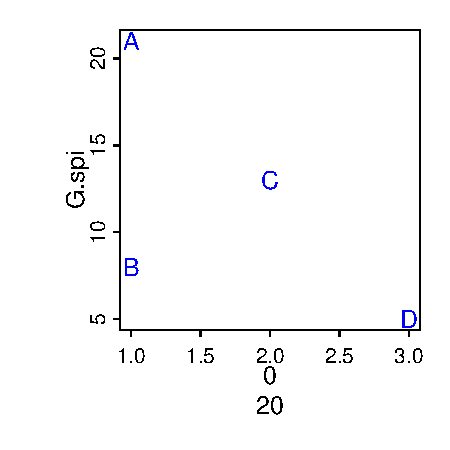
\includegraphics{02-Similitud_files/figure-latex/NMDS-1.pdf}
\caption{\label{fig:NMDS}Similitud de cuatro localidades hipotéticas}
\end{figure}

En la figura \ref{fig:NMDS} vemos que la composición de especies en el sitio A es diferente de la composición del sitio D. Es decir, la similitud entre el sitio A y D es menor que entre los otros sitios. Lo siguiente que nos deberíamos preguntar es; ¿qué tan similares son los dos sitios?

\hypertarget{uxedndices-cualitativos}{%
\subsection{Índices cualitativos}\label{uxedndices-cualitativos}}

Los índices cualitativos o de incidencia, son una medida que nos permite evaluar la similitud entre comunidades basados en presencia-ausencia de especies. A continuación veremos tres diferentes índices:

\begin{quote}
\[S_s= \frac{(2c)}{(a+b+2c)}\]
Índice de Sorensen

\[S_s= \frac{(c)}{(a+b+c)}\]
Índice de Jaccard

\[S_s= \frac{(c)}{c+min(a+b)}\]
Índice de Simpson
\end{quote}

Donde \emph{c} es el número de especies en común entre los dos sitios, \emph{a} y \emph{b} son el número de especies únicas en cada sitio. Las diferencias entre estos índices radica en la importancia que se le da a cada componente, en el caso del índice de Sorensen las especies compartidas tienen una gran importancia, por eso es multiplicada por dos. En el caso del índice de Simpson, es un índice usado cuando hay diferencias muy altas entre pares de comunidades, así restamos el peso obteniendo el valor mínimo de entre a y b.

Para calcular estos índices entre los sitios A y B necesitamos definir el número de especies compartidas y luego el número de especies únicas de los dos sitios.

\begin{Shaded}
\begin{Highlighting}[]
\NormalTok{comp }\OtherTok{\textless{}{-}}\NormalTok{ dens}
\NormalTok{comp[comp}\SpecialCharTok{\textgreater{}}\DecValTok{0}\NormalTok{] }\OtherTok{\textless{}{-}} \DecValTok{1} \CommentTok{\#Generamos una matriz de presencia ausencia}
\NormalTok{comp}
\end{Highlighting}
\end{Shaded}

\begin{verbatim}
##   T.bil G.spi C.tri C.sca
## A     1     1     1     1
## B     1     1     1     0
## C     1     1     1     1
## D     1     1     1     1
\end{verbatim}

\begin{Shaded}
\begin{Highlighting}[]
\NormalTok{a }\OtherTok{\textless{}{-}} \FunctionTok{sum}\NormalTok{(}\FunctionTok{colSums}\NormalTok{(comp[}\DecValTok{1}\SpecialCharTok{:}\DecValTok{2}\NormalTok{,])}\SpecialCharTok{==}\DecValTok{1}\SpecialCharTok{\&}\NormalTok{comp[}\DecValTok{2}\NormalTok{,]}\SpecialCharTok{==}\DecValTok{0}\NormalTok{)}\CommentTok{\#Ocurren en A pero no en B}
\NormalTok{b }\OtherTok{\textless{}{-}} \FunctionTok{sum}\NormalTok{(}\FunctionTok{colSums}\NormalTok{(comp[}\DecValTok{1}\SpecialCharTok{:}\DecValTok{2}\NormalTok{,])}\SpecialCharTok{==}\DecValTok{1}\SpecialCharTok{\&}\NormalTok{comp[}\DecValTok{1}\NormalTok{,]}\SpecialCharTok{==}\DecValTok{0}\NormalTok{)}\CommentTok{\#Ocurren en B pero no en A}
\NormalTok{c }\OtherTok{\textless{}{-}} \FunctionTok{sum}\NormalTok{(}\FunctionTok{colSums}\NormalTok{(comp[}\DecValTok{1}\SpecialCharTok{:}\DecValTok{2}\NormalTok{,])}\SpecialCharTok{==}\DecValTok{2}\NormalTok{) }\CommentTok{\#ocurren en A y B}

\NormalTok{a;b;c}
\end{Highlighting}
\end{Shaded}

\begin{verbatim}
## [1] 1
\end{verbatim}

\begin{verbatim}
## [1] 0
\end{verbatim}

\begin{verbatim}
## [1] 3
\end{verbatim}

Ahora obtenemos el valor de similitud entre los dos primeros sitios (A y B).

\begin{Shaded}
\begin{Highlighting}[]
\NormalTok{Sor }\OtherTok{\textless{}{-}}\NormalTok{ (}\DecValTok{2}\SpecialCharTok{*}\NormalTok{c)}\SpecialCharTok{/}\NormalTok{(a}\SpecialCharTok{+}\NormalTok{b}\SpecialCharTok{+}\NormalTok{(}\DecValTok{2}\SpecialCharTok{*}\NormalTok{c))}
\NormalTok{Jac }\OtherTok{\textless{}{-}}\NormalTok{ c}\SpecialCharTok{/}\NormalTok{(a}\SpecialCharTok{+}\NormalTok{b}\SpecialCharTok{+}\NormalTok{c)}
\NormalTok{Sim }\OtherTok{\textless{}{-}}\NormalTok{ c}\SpecialCharTok{/}\NormalTok{c}\SpecialCharTok{+}\FunctionTok{min}\NormalTok{(a,b)}

\NormalTok{Sor; Jac; Sim}
\end{Highlighting}
\end{Shaded}

\begin{verbatim}
## [1] 0.8571429
\end{verbatim}

\begin{verbatim}
## [1] 0.75
\end{verbatim}

\begin{verbatim}
## [1] 1
\end{verbatim}

Según el índice de Sorensen estos dos sitios son parecidos en un 86\%, mientras que para el índice de Jaccard es el 75\% y para Simpson estos dos sitios son iguales (100\%).

\hypertarget{uxedndices-cuantitativos}{%
\subsection{Índices cuantitativos}\label{uxedndices-cuantitativos}}

El \emph{porcentaje de similitud} es la versión cuantitativa del índice de Sorensen. Este índice está basado en datos de abundancia y es calculado como:

\begin{quote}
\[S_s= \frac{(2W)}{A+B}\]
Porcentaje de Similitud
\end{quote}

Donde; \emph{W} es la sumatoria del valor mínimo de la abundancia entre las comunidades comparadas para cada especie. \emph{A} y \emph{B} es la suma de las abundancias de todas las especies en cada sitio.

\begin{table}

\caption{\label{tab:unnamed-chunk-4}Medidas para obtener el porcentaje de Similitud}
\centering
\begin{tabular}[t]{l|r|r|r|r|r|l}
\hline
  & T.bil & G.spi & C.tri & C.sca & Medidas & Tipo\\
\hline
A & 1 & 21 & 11 & 16 & 49 & A\\
\hline
B & 1 & 8 & 3 & 0 & 12 & B\\
\hline
3 & 1 & 8 & 3 & 0 & 12 & W\\
\hline
\end{tabular}
\end{table}

\begin{Shaded}
\begin{Highlighting}[]
\NormalTok{PS }\OtherTok{\textless{}{-}}\NormalTok{ (}\DecValTok{2}\SpecialCharTok{*}\NormalTok{MatPS[}\DecValTok{3}\NormalTok{,}\DecValTok{5}\NormalTok{])}\SpecialCharTok{/}\NormalTok{(MatPS[}\DecValTok{1}\NormalTok{,}\DecValTok{5}\NormalTok{]}\SpecialCharTok{+}\NormalTok{MatPS[}\DecValTok{2}\NormalTok{,}\DecValTok{5}\NormalTok{])}
\NormalTok{PS}
\end{Highlighting}
\end{Shaded}

\begin{verbatim}
## [1] 0.3934426
\end{verbatim}

Esto significa que las comunidades A y B tienen un porcentaje de similitud del 39\%. Los datos de los dos tipos de índices utilizados difieren entre sí, el porcentaje de similitud utiliza no solamente la presencia-ausencia sino también la abundancia lo que podría estar reduciendo la similitud entre sitios.

\hypertarget{distancias-entre-sitios}{%
\section{Distancias entre sitios}\label{distancias-entre-sitios}}

Como hemos visto hasta ahora, cuando tenemos dos comunidades muy parecidas entre sí tendremos valores altos de similitud. En contraposición los índices de distancia nos mostrarán valores altos cuando dos comunidades se parezcan poco. Como habíamos mencionado anteriormente existen dos tipos de medidas de distancia;

\begin{itemize}
\item
  aquellas calculadas a partir de los índices de similitud usualmente como D= 1-Similitud. Así, para los índices de incidencia (presencia - ausencia) se pueden usar los índices de Jacard, Simpson o Sorensen, mientras que para los índices cuantitativos se puede usar el porcentaje de similitud, este último conocido como distancia de Bray Curtis.
\item
  aquellas que no tienen medidas de similitud análogas, algunos de estos índices son; Euclidiana, Chord, Hellinger.
\end{itemize}

La \emph{distancia} entre dos muestras está dada por la diferencia entre la abundancia y la composición de especies. En la figura \ref{fig:NMDS} se observa que la comunidad A esta más alejada de la comunidad D que de las otras dos.

\hypertarget{distancia-euclidiana}{%
\subsection{Distancia Euclidiana}\label{distancia-euclidiana}}

Existen muchas formas de poder calcular las distancias entre estas comunidades una de las más sencillas es la distancia \emph{Euclidiana}. La distancia euclidiana entre dos sitios es simplemente la longitud del vector que conecta los sitios y la podemos obtener como \(\sqrt{x^2+y^2}\), donde \emph{``x''} y \emph{``y''} son las coordenadas (x, y) de distancia entre un par de sitios.

En nuestro caso si queremos comparar B y C tenemos que la distancia en el eje \emph{x} es la diferencia de la abundancia de \emph{T. bilbergii} entre el sitio B y C.

\begin{Shaded}
\begin{Highlighting}[]
\NormalTok{x }\OtherTok{\textless{}{-}}\NormalTok{ dens[}\DecValTok{2}\NormalTok{, }\DecValTok{1}\NormalTok{] }\SpecialCharTok{{-}}\NormalTok{ dens[}\DecValTok{3}\NormalTok{, }\DecValTok{1}\NormalTok{]}
\end{Highlighting}
\end{Shaded}

Mientras que la distancia en el eje \emph{y} es la diferencia en la abundancia de \emph{G. spinosa} entre el sitio B y C.

\begin{Shaded}
\begin{Highlighting}[]
\NormalTok{y }\OtherTok{\textless{}{-}}\NormalTok{ dens[}\DecValTok{2}\NormalTok{, }\DecValTok{2}\NormalTok{] }\SpecialCharTok{{-}}\NormalTok{ dens[}\DecValTok{3}\NormalTok{, }\DecValTok{2}\NormalTok{]}
\end{Highlighting}
\end{Shaded}

Ahora obtenemos las distancias entre los dos sitios

\begin{Shaded}
\begin{Highlighting}[]
\FunctionTok{sqrt}\NormalTok{(x}\SpecialCharTok{\^{}}\DecValTok{2} \SpecialCharTok{+}\NormalTok{ y}\SpecialCharTok{\^{}}\DecValTok{2}\NormalTok{)}
\end{Highlighting}
\end{Shaded}

\begin{verbatim}
## [1] 5.09902
\end{verbatim}

Pero como en \emph{R} todo es sencillo podemos utilizar la función \emph{dist}

\begin{Shaded}
\begin{Highlighting}[]
\FunctionTok{dist}\NormalTok{(dens[,}\DecValTok{1}\SpecialCharTok{:}\DecValTok{2}\NormalTok{])}
\end{Highlighting}
\end{Shaded}

\begin{verbatim}
##           A         B         C
## B 13.000000                    
## C  8.062258  5.099020          
## D 16.124515  3.605551  8.062258
\end{verbatim}

Si bien este cálculo es sencillo con dos especies, si tenemos que calcular la distancia para una comunidad con más de tres especies los cálculos son tediosos y largos. Para calcular la distancia \emph{Euclidiana} entre pares de sitios con \emph{R} especies utilizamos la siguiente ecuación:

\begin{quote}
\[D_E = \sqrt{\sum_{i=l}^R (x_{ai} - x_{bi})^2}\]
Distancia Euclidiana
\end{quote}

\hypertarget{efecto-de-doble-ceros-y-abundancia}{%
\subsubsection{Efecto de doble-ceros y abundancia}\label{efecto-de-doble-ceros-y-abundancia}}

Aunque la distancia Euclidiana es fácilmente interpretable, es poco usado en análisis biológicos. Normalmente los datos de comunidad están caracterizados por una gran cantidad de ceros (especies no encontradas en determinados sitios), el cálculo de la distancia Euclidiana incrementa la similitud entre comunidades que presentan ceros para la misma especie.

\begin{table}

\caption{\label{tab:unnamed-chunk-10}Efecto del doble cero}
\centering
\begin{tabular}[t]{l|r|r|r|r|r|r}
\hline
  & spp1 & spp2 & spp3 & sp4 & spp5 & spp6\\
\hline
A & 1 & 1 & 0 & 0 & 0 & 0\\
\hline
B & 0 & 1 & 1 & 1 & 1 & 0\\
\hline
C & 0 & 0 & 0 & 0 & 1 & 1\\
\hline
\end{tabular}
\end{table}

Según los datos mostrados en la tabla tendríamos que hay un gradiente, la comunidad A comparte una especie con la comunidad B y la comunidad B comparte una especie con la comunidad C. Los índices deberían permitir recuperar ese gradiente, veamos lo que pasa.

\begin{Shaded}
\begin{Highlighting}[]
\FunctionTok{library}\NormalTok{(vegan)}
\end{Highlighting}
\end{Shaded}

\begin{verbatim}
## Loading required package: permute
\end{verbatim}

\begin{verbatim}
## Loading required package: lattice
\end{verbatim}

\begin{verbatim}
## This is vegan 2.5-7
\end{verbatim}

\begin{Shaded}
\begin{Highlighting}[]
\FunctionTok{vegdist}\NormalTok{(dcMat, }\StringTok{"euclidean"}\NormalTok{)}
\end{Highlighting}
\end{Shaded}

\begin{verbatim}
##   A B
## B 2  
## C 2 2
\end{verbatim}

Como vemos en el ejemplo, el doble cero de la comunidad A y C generan una mayor similitud, de esta forma, las tres comunidades son mostradas a igual distancia.

Esto no debería ser un problema si el cero nos diese información consistente. En el caso de datos biológicos el tener un valor de cero puede deberse a varias razones, por ejemplo puede ser que aunque la especie ocurre en ese lugar no pudo ser muestreada, o realmente no ocurre en ese lugar por restricciones abióticas, de esta forma el cero no es informativo y no podemos usarlo para generar matrices de distancias. En otros casos, normalmente en datos abióticos, el cero implica la ausencia de algo, por ejemplo tener cero mg de un contaminante es una información. De esta forma la distancia Euclidiana es usada sobre todo para interpretar datos ambientales.

\hypertarget{efecto-de-la-abundancia}{%
\subsubsection{Efecto de la abundancia}\label{efecto-de-la-abundancia}}

Otra característica importante de la distancia euclidiana es que está fuertemente impactada por la diferencia de abundancias entre especies. El cálculo de esta distancia eleva al cuadrado las abundancias, por lo que el impacto de las especies dominantes es desproporcionado. En otras palabras la distancia euclideana incrementa el efecto de las especies dominantes. Veamos a qué nos referimos en el siguiente ejemplo.

\begin{Shaded}
\begin{Highlighting}[]
\NormalTok{dcMat2 }\OtherTok{\textless{}{-}} \FunctionTok{data.frame}\NormalTok{(}\AttributeTok{spp1=}\FunctionTok{c}\NormalTok{(}\DecValTok{0}\NormalTok{,}\DecValTok{1}\NormalTok{,}\DecValTok{0}\NormalTok{),}\AttributeTok{spp2=}\FunctionTok{c}\NormalTok{(}\DecValTok{1}\NormalTok{,}\DecValTok{0}\NormalTok{,}\DecValTok{8}\NormalTok{),}
                    \AttributeTok{spp3=}\FunctionTok{c}\NormalTok{(}\DecValTok{1}\NormalTok{,}\DecValTok{0}\NormalTok{,}\DecValTok{7}\NormalTok{))}

\FunctionTok{rownames}\NormalTok{(dcMat2) }\OtherTok{\textless{}{-}}\NormalTok{ LETTERS[}\DecValTok{1}\SpecialCharTok{:}\DecValTok{3}\NormalTok{]}

\FunctionTok{kable}\NormalTok{(dcMat2, }\AttributeTok{caption =} \StringTok{"Efecto de la abundancia"}\NormalTok{)}
\end{Highlighting}
\end{Shaded}

\begin{table}

\caption{\label{tab:unnamed-chunk-12}Efecto de la abundancia}
\centering
\begin{tabular}[t]{l|r|r|r}
\hline
  & spp1 & spp2 & spp3\\
\hline
A & 0 & 1 & 1\\
\hline
B & 1 & 0 & 0\\
\hline
C & 0 & 8 & 7\\
\hline
\end{tabular}
\end{table}

\begin{Shaded}
\begin{Highlighting}[]
\FunctionTok{vegdist}\NormalTok{(dcMat2, }\StringTok{"euclidean"}\NormalTok{)}
\end{Highlighting}
\end{Shaded}

\begin{verbatim}
##           A         B
## B  1.732051          
## C  9.219544 10.677078
\end{verbatim}

Como vemos la distancia de la comunidad A a la C es de 9.21, aunque comparten dos especies, la diferencia en abundancias entre estas dos comunidades es muy marcada generando un incremento en la distancia. Por otro lado, la comunidad A tiene una distancia de 1.73 a la comunidad B, esta menor distancia se da aunque no comparten ninguna especie. Como vemos el efecto en la diferencia de abundancias tiene un fuerte impacto sobre el cálculo de distancias.

\hypertarget{distancia-bray-curtis}{%
\subsection{Distancia Bray-Curtis}\label{distancia-bray-curtis}}

Existen otras formas de medir distancias entre dos localidades. En ecología una de las distancias más utilizada es la de \emph{Bray-Curtis}, esta distancia es el opuesto del porcentaje de similitud, que a su vez es la versión de abundancia del índice de Sorensen. Esta distancia es calculada como:

\begin{quote}
\[D_{BC} = \sum_{i=l}^R \frac{(x_{ai} - x_{bi})}{(x_{ai} + x_{bi})}\]
Distancia de Bray-Curtis
\end{quote}

La distancia \emph{Bray-Curtis} se refiere a la diferencia total en la abundancia de especies entre dos sitios, dividido para la abundancia total en cada sitio. La distancia Bray-Curtis tiende a resultar más intuitiva debido a que las especies comunes y raras tienen pesos relativamente similares, mientras que la distancia euclidiana depende en mayor medida de las especies más abundantes. Esto sucede porque las distancias euclidianas se basan en diferencias al cuadrado, mientras que Bray-Curtis utiliza diferencias absolutas. El elevar un número al cuadrado siempre amplifica la importancia de los valores más grandes. En la figura \ref{fig:bray} se compara gráficos basados en distancias euclidianas y Bray-Curtis de los mismos datos.

Como se había comentado, es virtualmente imposible representar una distancia en más de tres dimensiones (cada especie es una dimensión). Una forma sencilla de mostrar distancias para tres o más especies es crear un gráfico de dos dimensiones, intentando organizar todos los sitios para que las distancias sean aproximadamente las correctas. Está claro que esto es una aproximación, las distancias nunca serán exactas. Una técnica que intenta crear un arreglo aproximado es escalamiento multidimensional no métrico (NMDS).

La función de escalamiento multidimensional no-métrico está en el paquete \texttt{vegan}. Aquí mostramos las distancias euclidianas entre sitios (Figura \ref{fig:bray}a) y las distancias de Bray-Curtis (Figura \ref{fig:bray}b).

\begin{Shaded}
\begin{Highlighting}[]
\FunctionTok{library}\NormalTok{(vegan) }

\CommentTok{\#Distancia Euclidiana}
\NormalTok{mdsE }\OtherTok{\textless{}{-}} \FunctionTok{metaMDS}\NormalTok{(dcMat, }\AttributeTok{distance =} \StringTok{"euc"}\NormalTok{, }\AttributeTok{autotransform =} \ConstantTok{FALSE}\NormalTok{, }\AttributeTok{trace =} \DecValTok{0}\NormalTok{) }
\CommentTok{\#Distancia de Bray{-}Curtis}
\NormalTok{mdsB }\OtherTok{\textless{}{-}} \FunctionTok{metaMDS}\NormalTok{(dcMat, }\AttributeTok{distance =} \StringTok{"bray"}\NormalTok{, }\AttributeTok{autotransform =} \ConstantTok{FALSE}\NormalTok{, }\AttributeTok{trace =} \DecValTok{0}\NormalTok{) }
\end{Highlighting}
\end{Shaded}

\begin{Shaded}
\begin{Highlighting}[]
\FunctionTok{par}\NormalTok{(}\AttributeTok{mfcol=}\FunctionTok{c}\NormalTok{(}\DecValTok{1}\NormalTok{,}\DecValTok{2}\NormalTok{), }\AttributeTok{oma=}\FunctionTok{c}\NormalTok{(}\DecValTok{1}\NormalTok{,}\DecValTok{1}\NormalTok{,}\DecValTok{1}\NormalTok{,}\DecValTok{1}\NormalTok{), }\AttributeTok{mar=}\FunctionTok{c}\NormalTok{(}\DecValTok{4}\NormalTok{,}\DecValTok{4}\NormalTok{,}\DecValTok{1}\NormalTok{,}\DecValTok{1}\NormalTok{),}
    \AttributeTok{mgp=}\FunctionTok{c}\NormalTok{(}\DecValTok{1}\NormalTok{,}\FloatTok{0.3}\NormalTok{,}\DecValTok{0}\NormalTok{), }\AttributeTok{tcl=} \SpecialCharTok{{-}}\FloatTok{0.2}\NormalTok{)}

\FunctionTok{plot}\NormalTok{(mdsE, }\AttributeTok{display =} \StringTok{"sites"}\NormalTok{, }
     \AttributeTok{type =} \StringTok{"text"}\NormalTok{,}\AttributeTok{main=}\StringTok{"a)Euclidiana"}\NormalTok{, }
     \AttributeTok{cex.axis=} \FloatTok{0.7}\NormalTok{, }\AttributeTok{cex.main=}\FloatTok{0.75}\NormalTok{, }\AttributeTok{cex.lab=}\FloatTok{0.7}\NormalTok{)}

\FunctionTok{plot}\NormalTok{(mdsB, }\AttributeTok{display =} \StringTok{"sites"}\NormalTok{, }\AttributeTok{type =} \StringTok{"text"}\NormalTok{, }
     \AttributeTok{main=}\StringTok{"b)Bray{-}Curtis"}\NormalTok{, }
     \AttributeTok{cex.axis=} \FloatTok{0.7}\NormalTok{, }\AttributeTok{cex.main=}\FloatTok{0.75}\NormalTok{, }\AttributeTok{cex.lab=}\FloatTok{0.7}\NormalTok{)}
\end{Highlighting}
\end{Shaded}

\begin{figure}
\centering
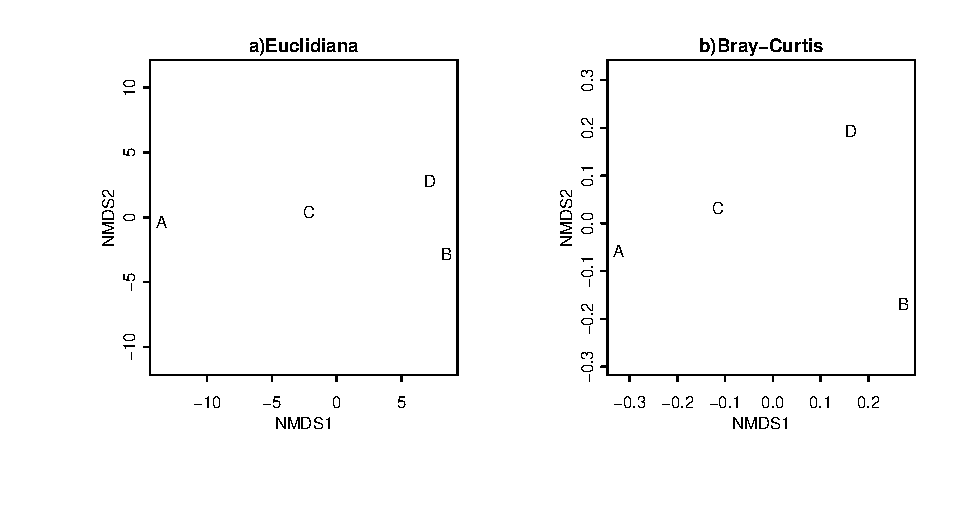
\includegraphics{02-Similitud_files/figure-latex/bray-1.pdf}
\caption{\label{fig:bray}Arreglo de las parcelas en distancias multidimensionales no métricas (NMDS). Estas dos figuras muestran los mismos datos en bruto, pero las distancias euclidianas tienden a enfatizar las diferencias debidas a las especies más abundantes, mientras que Bray-Curtis no lo hace.}
\end{figure}

Como podemos apreciar en el caso del ejemplo, la distancia de Bray-Curtis recupera la idea de un gradiente entre las comunidades, desde la comunidad A a la C. En el caso de la distancia Euclidiana las comunidades B y C se encuentran a igual distancia de la comunidad A, como un efecto del doble cero.

\hypertarget{transformaciuxf3n-y-estandarizaciuxf3n-de-datos}{%
\section{Transformación y Estandarización de datos}\label{transformaciuxf3n-y-estandarizaciuxf3n-de-datos}}

Cuando trabajamos con datos multivariantes cabe la posibilidad de que los datos dentro de esta matriz tengan diferencias de magnitud importantes. Como vimos antes el cálculo de distancia entre los sitios puede verse fuertemente afectado por la magnitud de sus diferencias.

En el ejemplo que mostramos en el inicio, las similitudes entre comunidades basadas en las dos primeras especies, las diferencias entre las comunidades depende de la escala de medición (los valores de los ejes), y sobre cómo medimos la distancia a través del espacio multivariado \citep{Stevens2009}.

De esta forma, las diferencias entre sitios son dependientes de la abundancia de cada especie. En el caso de \emph{G. spinosa} su eje varía entre 5 y 21, mientras que para \emph{T. billbergii} varía entre 1 y 3 (Figura \ref{fig:NMDS2}a). Veamos ahora que sucede con las similitud si incremento la abundancia de \emph{T. billbergii} (Figura \ref{fig:NMDS2}b).

\begin{Shaded}
\begin{Highlighting}[]
\FunctionTok{par}\NormalTok{(}\AttributeTok{mar=}\FunctionTok{c}\NormalTok{(}\DecValTok{4}\NormalTok{,}\DecValTok{4}\NormalTok{,}\DecValTok{1}\NormalTok{,}\DecValTok{1}\NormalTok{), }\AttributeTok{mgp=}\FunctionTok{c}\NormalTok{(}\DecValTok{1}\NormalTok{,}\FloatTok{0.3}\NormalTok{,}\DecValTok{0}\NormalTok{), }\AttributeTok{mfcol=}\FunctionTok{c}\NormalTok{(}\DecValTok{1}\NormalTok{,}\DecValTok{2}\NormalTok{), }\AttributeTok{tcl=} \SpecialCharTok{{-}}\FloatTok{0.2}\NormalTok{)}
\NormalTok{dens1 }\OtherTok{\textless{}{-}}\NormalTok{ dens}
\NormalTok{dens1}\SpecialCharTok{$}\NormalTok{T.bil }\OtherTok{\textless{}{-}}\NormalTok{ dens1}\SpecialCharTok{$}\NormalTok{T.bil}\SpecialCharTok{*}\DecValTok{100}
\FunctionTok{plot}\NormalTok{(dens[,}\DecValTok{1}\SpecialCharTok{:}\DecValTok{2}\NormalTok{], }\AttributeTok{type =} \StringTok{"n"}\NormalTok{, }\AttributeTok{cex.axis=}\FloatTok{0.8}\NormalTok{, }\AttributeTok{xlim=}\FunctionTok{c}\NormalTok{(}\DecValTok{0}\NormalTok{,}\DecValTok{30}\NormalTok{), }\AttributeTok{ylim=}\FunctionTok{c}\NormalTok{(}\DecValTok{0}\NormalTok{,}\DecValTok{30}\NormalTok{), }\AttributeTok{main=}\StringTok{"a."}\NormalTok{) }
\FunctionTok{text}\NormalTok{(dens[,}\DecValTok{1}\SpecialCharTok{:}\DecValTok{2}\NormalTok{], }\FunctionTok{row.names}\NormalTok{(dens), }\AttributeTok{col =}\StringTok{"blue"}\NormalTok{)}

\FunctionTok{plot}\NormalTok{(dens1[,}\DecValTok{1}\SpecialCharTok{:}\DecValTok{2}\NormalTok{], }\AttributeTok{type =} \StringTok{"n"}\NormalTok{, }\AttributeTok{cex.axis=}\FloatTok{0.8}\NormalTok{, }\AttributeTok{ylim=}\FunctionTok{c}\NormalTok{(}\DecValTok{0}\NormalTok{,}\DecValTok{300}\NormalTok{), }\AttributeTok{main=}\StringTok{"b."}\NormalTok{) }
\FunctionTok{text}\NormalTok{(dens1[,}\DecValTok{1}\SpecialCharTok{:}\DecValTok{2}\NormalTok{], }\FunctionTok{row.names}\NormalTok{(dens1), }\AttributeTok{col =}\StringTok{"blue"}\NormalTok{)}
\end{Highlighting}
\end{Shaded}

\begin{figure}
\centering
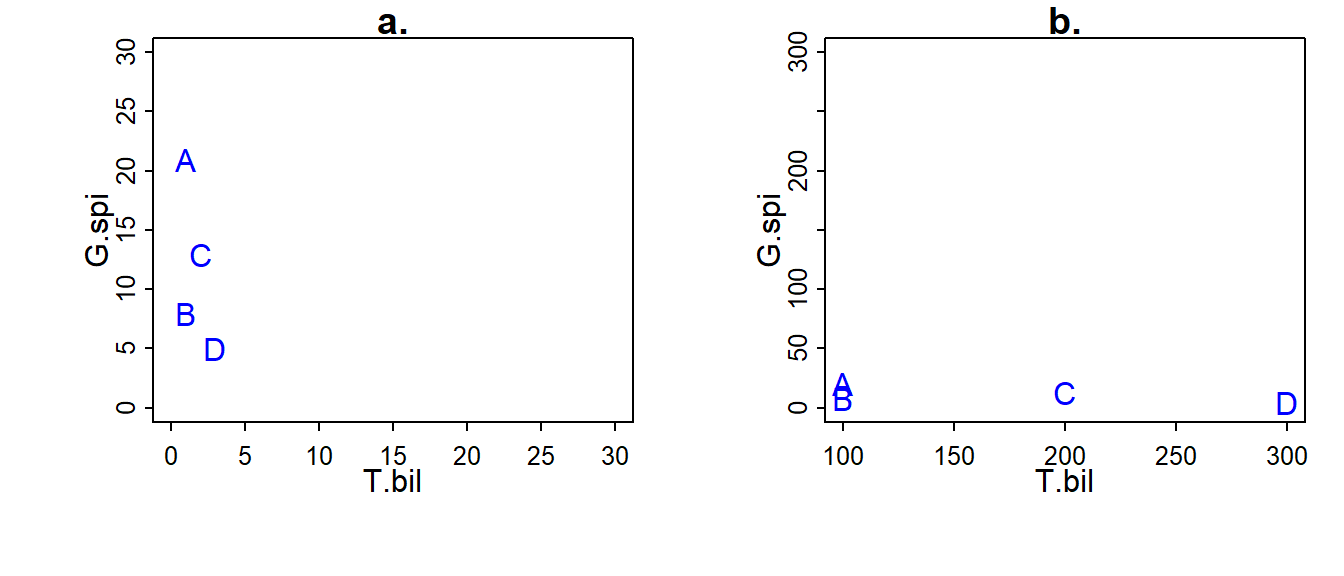
\includegraphics{02-Similitud_files/figure-latex/NMDS2-1.pdf}
\caption{\label{fig:NMDS2}Distancias de cuatro localidades hipotéticas}
\end{figure}

Como vemos en la figura \ref{fig:NMDS2} las distancias entre cada uno de los sitios cambio cuando incremento la abundancia de \emph{T. bilbergi}, aunque este incremento fue proporcional. Una forma de corregir esta distorsión es calcular la densidad relativa de cada especie, de esta forma cada especie variará entre 0 y 1 \citep{Stevens2009}. Cuando nos referimos a densidad relativa hablamos de la densidad de una especie con referencia a algo, en este caso con relación a la abundancia de individuos de la misma especie en otros sitios.

Para calcular la densidad relativa dividimos la abundancia de cada especie para la suma total de los individuos de las especies en esa muestra.

\begin{Shaded}
\begin{Highlighting}[]
\NormalTok{dens[,}\DecValTok{1}\NormalTok{]}\SpecialCharTok{/}\FunctionTok{sum}\NormalTok{(dens[,}\DecValTok{1}\NormalTok{])}
\end{Highlighting}
\end{Shaded}

\begin{verbatim}
## [1] 0.1428571 0.1428571 0.2857143 0.4285714
\end{verbatim}

\begin{Shaded}
\begin{Highlighting}[]
\NormalTok{dens1[,}\DecValTok{1}\NormalTok{]}\SpecialCharTok{/}\FunctionTok{sum}\NormalTok{(dens1[,}\DecValTok{1}\NormalTok{])}
\end{Highlighting}
\end{Shaded}

\begin{verbatim}
## [1] 0.1428571 0.1428571 0.2857143 0.4285714
\end{verbatim}

Ahora podemos ver cómo \emph{T. billbergii} varía en su abundancia en los cuatro sitios. Los sitios A y B tienen el 14\% de individuos mientras que el D tiene el 42\% de los individuos de esta especie. Interesantemente, no hay diferencias en las proporciones entre las dos medidas que tenemos. ¿Qué pasó con las distancias?

\begin{figure}
\centering
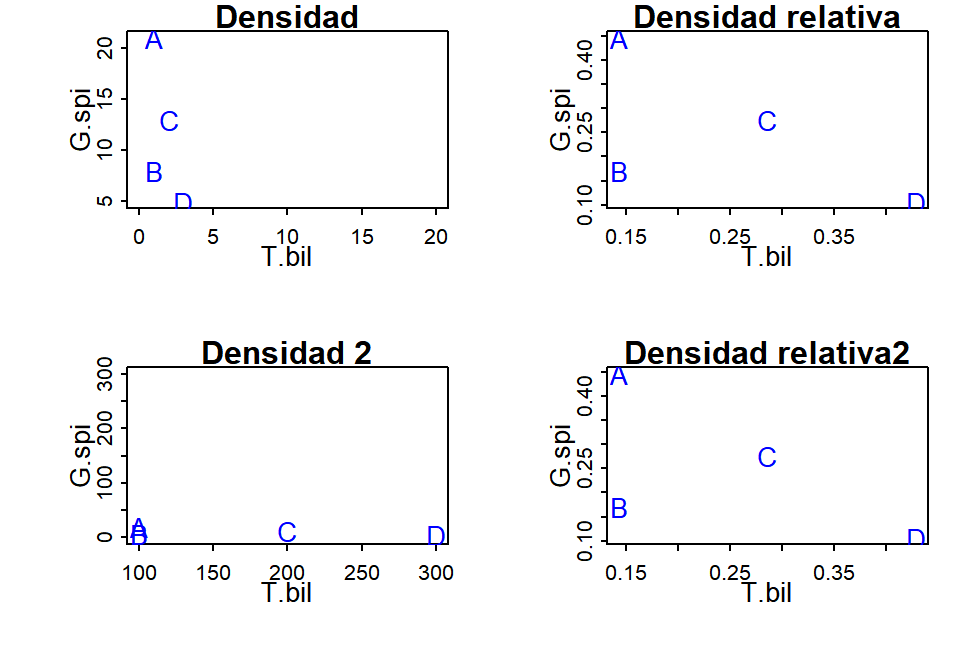
\includegraphics{02-Similitud_files/figure-latex/NMDS3-1.pdf}
\caption{\label{fig:NMDS3}Distancias de cuatro localidades hipotéticas}
\end{figure}

En la figura \ref{fig:NMDS3} podemos apreciar que no hay diferencias entre las dos densidades cuando estoy usando la densidad relativa. Pero ¿Qué implicaciones biológicas tiene el usar las densidades relativas para calcular la distancia entre sitios?

Cuando usamos las densidades relativas estamos dando el mismo peso a todas las especies. En un ecosistema con una especie dominante y varias subordinadas, al usar la densidad relativa estoy eliminando esa dominancia. Es importante tener claro este punto, ya que las interpretaciones que puedo hacer con los datos de abundancia y abundancia relativa son distintos.

\hypertarget{transformaciuxf3n-de-datos}{%
\subsection{Transformación de datos}\label{transformaciuxf3n-de-datos}}

Esta claro que la magnitud de las diferencias entre las variables tiene un impacto sobre el cálculo de la distancia. Ahora, nos interesa poder manejar el efecto de esas diferencias, para lo cual desarrollamos una transformación.

La transformación de datos implica una modificación de los datos brutos a través de una ecuación algebraica. La transformación de datos implica una modificación independientemente para cada dato, no existe influencia del resto de datos.

\begin{table}

\caption{\label{tab:unnamed-chunk-16}Comunidad de macroinvertebrados acuáticos}
\centering
\begin{tabular}[t]{l|r|r|r|r|r|r|r|r|r|r|r}
\hline
LOCALIDAD & Allu & Atop & Atri & Baet & Bezz & Blep & Cera & Chel & Chim & Chir & Cole\\
\hline
Bo-1 & 0 & 0 & 0 & 6 & 0 & 1 & 0 & 1 & 3 & 18 & 4\\
\hline
Bo-2 & 0 & 0 & 0 & 3 & 0 & 0 & 0 & 0 & 1 & 9 & 0\\
\hline
Bo-3 & 0 & 0 & 0 & 6 & 0 & 0 & 1 & 1 & 1 & 9 & 0\\
\hline
BP-1 & 0 & 3 & 0 & 81 & 0 & 0 & 0 & 0 & 0 & 27 & 0\\
\hline
BP-2 & 0 & 0 & 0 & 9 & 0 & 0 & 0 & 0 & 2 & 0 & 0\\
\hline
BP-3 & 0 & 0 & 0 & 54 & 0 & 0 & 1 & 0 & 0 & 9 & 0\\
\hline
Pa-1 & 1 & 0 & 0 & 984 & 0 & 0 & 0 & 0 & 0 & 81 & 0\\
\hline
Pa-2 & 0 & 0 & 0 & 15 & 0 & 0 & 0 & 0 & 1 & 9 & 0\\
\hline
Pa-3 & 0 & 0 & 0 & 93 & 1 & 0 & 0 & 0 & 0 & 18 & 0\\
\hline
Ur-1 & 0 & 0 & 0 & 6 & 0 & 0 & 0 & 0 & 0 & 855 & 0\\
\hline
Ur-2 & 0 & 0 & 1 & 12 & 0 & 0 & 0 & 1 & 0 & 9 & 0\\
\hline
Ur-3 & 0 & 0 & 0 & 0 & 10 & 0 & 0 & 0 & 0 & 27 & 0\\
\hline
\end{tabular}
\end{table}

En la tabla anterior podemos ver que la comunidad está compuesta por un par de especies dominantes y varias especies raras.

Al transformar los datos evitamos que las especies dominantes definan el cálculo de la distancia.

Existen varias posibilidades para transformar los datos, por lo que definir que función utilizar es importante. Cada tipo de transformación produce resultados distintos por lo que debemos utilizarlas con precaución.

La transformación más sencilla o menos intensa es la raíz cuadrada, mientras que el logaritmo es la transformación más intensa, podríamos utilizar la raíz cuarta como una función intermedia. La raíz cuadrada la utilizaríamos cuando tenemos diferencias con variaciones de una magnitud de diferencia (entre decenas y centenas), mientras que la transformación logarítmica la haríamos con comunidades donde hay más de una magnitud de diferencia (entre decenas y miles).

Aunque hay muchos autores que aconsejan realizar transformaciones hay que ser conscientes de lo que estamos haciendo, transformaciones muy fuertes en una matriz con pocas diferencias pueden hacer que, por ejemplo, las especies raras tengan igual peso que las dominantes, ¿esto es lo que queremos?

\textbf{Recuerde: las diferentes transformaciones tienen interpretaciones biológicas distintas. Debemos ser conscientes de lo que estamos haciendo y de su posterior interpretación biológica.}

Veamos un ejemplo:

\begin{Shaded}
\begin{Highlighting}[]
\FunctionTok{set.seed}\NormalTok{(}\DecValTok{4}\NormalTok{)}
\NormalTok{aves}\OtherTok{\textless{}{-}} \FunctionTok{data.frame}\NormalTok{(}\AttributeTok{sp1=} \FunctionTok{sample}\NormalTok{(}\DecValTok{1}\SpecialCharTok{:}\DecValTok{90}\NormalTok{, }\DecValTok{10}\NormalTok{), }\AttributeTok{sp2=} \FunctionTok{sample}\NormalTok{(}\DecValTok{100}\SpecialCharTok{:}\DecValTok{250}\NormalTok{, }\DecValTok{10}\NormalTok{))}

\NormalTok{insectos}\OtherTok{\textless{}{-}} \FunctionTok{data.frame}\NormalTok{(}\AttributeTok{sp1=} \FunctionTok{sample}\NormalTok{(}\DecValTok{5}\SpecialCharTok{:}\DecValTok{99}\NormalTok{, }\DecValTok{10}\NormalTok{), }\AttributeTok{sp2=} \FunctionTok{sample}\NormalTok{(}\DecValTok{1000}\SpecialCharTok{:}\DecValTok{2500}\NormalTok{, }\DecValTok{10}\NormalTok{))}

\DocumentationTok{\#\#¿Qué pasa cuando transformamos?}
\NormalTok{aveT }\OtherTok{\textless{}{-}} \FunctionTok{round}\NormalTok{(}\FunctionTok{cbind}\NormalTok{(aves, }\FunctionTok{sqrt}\NormalTok{(aves),}\FunctionTok{log}\NormalTok{(aves)),}\DecValTok{2}\NormalTok{)}
\FunctionTok{colnames}\NormalTok{(aveT) }\OtherTok{\textless{}{-}} \FunctionTok{paste}\NormalTok{(}\FunctionTok{rep}\NormalTok{(}\FunctionTok{c}\NormalTok{(}\StringTok{"sp1"}\NormalTok{, }\StringTok{"sp2"}\NormalTok{), }\DecValTok{3}\NormalTok{), }\FunctionTok{c}\NormalTok{(}\StringTok{""}\NormalTok{,}\StringTok{""}\NormalTok{,}\StringTok{"sqrt"}\NormalTok{, }\StringTok{"sqrt"}\NormalTok{, }\StringTok{"log"}\NormalTok{, }\StringTok{"log"}\NormalTok{), }\AttributeTok{sep=}\StringTok{"."}\NormalTok{)}

\FunctionTok{kable}\NormalTok{(aveT, }\AttributeTok{caption =} \StringTok{"Efecto de la transformación. Pequeñas diferencias"}\NormalTok{)}
\end{Highlighting}
\end{Shaded}

\begin{table}

\caption{\label{tab:unnamed-chunk-17}Efecto de la transformación. Pequeñas diferencias}
\centering
\begin{tabular}[t]{r|r|r|r|r|r}
\hline
sp1. & sp2. & sp1.sqrt & sp2.sqrt & sp1.log & sp2.log\\
\hline
75 & 201 & 8.66 & 14.18 & 4.32 & 5.30\\
\hline
51 & 229 & 7.14 & 15.13 & 3.93 & 5.43\\
\hline
3 & 228 & 1.73 & 15.10 & 1.10 & 5.43\\
\hline
71 & 183 & 8.43 & 13.53 & 4.26 & 5.21\\
\hline
44 & 134 & 6.63 & 11.58 & 3.78 & 4.90\\
\hline
58 & 208 & 7.62 & 14.42 & 4.06 & 5.34\\
\hline
89 & 147 & 9.43 & 12.12 & 4.49 & 4.99\\
\hline
56 & 200 & 7.48 & 14.14 & 4.03 & 5.30\\
\hline
30 & 224 & 5.48 & 14.97 & 3.40 & 5.41\\
\hline
62 & 249 & 7.87 & 15.78 & 4.13 & 5.52\\
\hline
\end{tabular}
\end{table}

\begin{Shaded}
\begin{Highlighting}[]
\NormalTok{insT }\OtherTok{\textless{}{-}} \FunctionTok{round}\NormalTok{(}\FunctionTok{cbind}\NormalTok{(insectos, }\FunctionTok{sqrt}\NormalTok{(insectos),}\FunctionTok{log}\NormalTok{(insectos)),}\DecValTok{2}\NormalTok{) }
\FunctionTok{colnames}\NormalTok{(insT) }\OtherTok{\textless{}{-}} \FunctionTok{paste}\NormalTok{(}\FunctionTok{rep}\NormalTok{(}\FunctionTok{c}\NormalTok{(}\StringTok{"sp1"}\NormalTok{, }\StringTok{"sp2"}\NormalTok{), }\DecValTok{3}\NormalTok{), }\FunctionTok{c}\NormalTok{(}\StringTok{""}\NormalTok{,}\StringTok{""}\NormalTok{,}\StringTok{"sqrt"}\NormalTok{, }\StringTok{"sqrt"}\NormalTok{, }\StringTok{"log"}\NormalTok{, }\StringTok{"log"}\NormalTok{), }\AttributeTok{sep=}\StringTok{"."}\NormalTok{)}

\FunctionTok{kable}\NormalTok{(insT, }\AttributeTok{caption =} \StringTok{"Efecto de la transformación, Grandes diferencias"}\NormalTok{)}
\end{Highlighting}
\end{Shaded}

\begin{table}

\caption{\label{tab:unnamed-chunk-17}Efecto de la transformación, Grandes diferencias}
\centering
\begin{tabular}[t]{r|r|r|r|r|r}
\hline
sp1. & sp2. & sp1.sqrt & sp2.sqrt & sp1.log & sp2.log\\
\hline
36 & 1202 & 6.00 & 34.67 & 3.58 & 7.09\\
\hline
51 & 2428 & 7.14 & 49.27 & 3.93 & 7.79\\
\hline
48 & 2088 & 6.93 & 45.69 & 3.87 & 7.64\\
\hline
73 & 1303 & 8.54 & 36.10 & 4.29 & 7.17\\
\hline
19 & 1151 & 4.36 & 33.93 & 2.94 & 7.05\\
\hline
26 & 1891 & 5.10 & 43.49 & 3.26 & 7.54\\
\hline
96 & 2338 & 9.80 & 48.35 & 4.56 & 7.76\\
\hline
68 & 1396 & 8.25 & 37.36 & 4.22 & 7.24\\
\hline
53 & 1979 & 7.28 & 44.49 & 3.97 & 7.59\\
\hline
58 & 2339 & 7.62 & 48.36 & 4.06 & 7.76\\
\hline
\end{tabular}
\end{table}

\hypertarget{estandarizaciuxf3n-de-los-datos}{%
\subsection{Estandarización de los datos}\label{estandarizaciuxf3n-de-los-datos}}

La estandarización de los datos permite modificar las variables transformándolas en unidades de desviación típica, lo que nos permite comparar entre valores de distribuciones normales diferentes, o de valores diferentes.

La estandarización o tipificación se lo realiza restando a cada valor el valor medio de la variable y dividiendo para la desviación estándar.

\begin{Shaded}
\begin{Highlighting}[]
\NormalTok{avesE }\OtherTok{\textless{}{-}}\NormalTok{ (aves[,}\DecValTok{1}\NormalTok{]}\SpecialCharTok{{-}}\FunctionTok{mean}\NormalTok{(aves[,}\DecValTok{1}\NormalTok{]))}\SpecialCharTok{/}\FunctionTok{sd}\NormalTok{(aves[,}\DecValTok{1}\NormalTok{])}
\NormalTok{avesE}
\end{Highlighting}
\end{Shaded}

\begin{verbatim}
##  [1]  0.86745705 -0.11922395 -2.09258597  0.70301022 -0.40700592  0.16855801
##  [7]  1.44302097  0.08633459 -0.98256984  0.33300484
\end{verbatim}

\begin{Shaded}
\begin{Highlighting}[]
\FunctionTok{round}\NormalTok{(}\FunctionTok{mean}\NormalTok{(avesE),}\DecValTok{1}\NormalTok{);}\FunctionTok{sd}\NormalTok{(avesE) }
\end{Highlighting}
\end{Shaded}

\begin{verbatim}
## [1] 0
\end{verbatim}

\begin{verbatim}
## [1] 1
\end{verbatim}

Como vemos las variables estandarizadas tienen como propiedad que la desviación estándar es 1 y la media es 0.

\begin{center}\rule{0.5\linewidth}{0.5pt}\end{center}

\hypertarget{ejercicio-pruxe1ctico}{%
\section{Ejercicio práctico}\label{ejercicio-pruxe1ctico}}

\begin{center}\rule{0.5\linewidth}{0.5pt}\end{center}

Una de las preguntas básicas de un ecólogo es saber ¿Cómo de diferentes son dos comunidades?. Como hemos visto existen varias decisiones que los investigadores debemos tomar, estas decisiones afectan directamente a los resultados que podemos obtener y por ende a las conclusiones biológicas que obtenemos de este análisis.

En el presente ejercicio evaluaremos cómo las diferentes decisiones que tomamos entorno al procesamiento de datos afectan nuestras medidas de similitud, y cuáles son las conclusiones biológicas que obtenemos con uno u otro procedimiento. En la tabla \ref{tab:ejer1} mostramos cinco comunidades hipotéticas.

\begin{table}

\caption{\label{tab:ejer1}Comunidades hipotéticas}
\centering
\begin{tabular}[t]{lrrrrrrrr}
\toprule
  & sp1 & sp2 & sp3 & sp4 & sp5 & sp6 & sp7 & sp8\\
\midrule
A & 58 & 58 & 11 & 1297 & 34 & 15 & 436 & 174\\
B & 52 & 23 & 29 & 1572 & 56 & 0 & 293 & 65\\
C & 0 & 0 & 36 & 41 & 85 & 0 & 449 & 91\\
D & 64 & 82 & 30 & 1300 & 46 & 45 & 454 & 209\\
E & 62 & 88 & 116 & 146 & 150 & 53 & 487 & 157\\
\bottomrule
\end{tabular}
\end{table}

Convierta los datos de abundancia brindados en la tabla \ref{tab:ejer1} en datos de abundancia relativa por cada sitio (la suma en cada sitio debe ser igual a 1). Dibuje dos gráficas para representar; i) la abundancia total y ii) abundancia relativa de cada localidad. En el ejercicio hemos calculado la abundancia relativa por especie y no por sitio. Para obtener la abundancia relativa por sitio use la siguiente línea de código:

\begin{verbatim}
objeto/rowSums(objeto)
\end{verbatim}

Para realizar los gráficos con los datos de abundancia y abundancia relativa use la función \emph{barplot} siguiendo la siguiente línea de código:

\begin{verbatim}
par(mfcol=c(2,1), mar=c(3,3,1,1))
barplot(objeto, beside = T)
barplot(objeto2, beside = T)
\end{verbatim}

La función \emph{par} se usa para dividir el área del gráfico en dos partes.

\begin{quote}
objeto y objeto2 se refiere al objeto que contiene la matriz de con los datos de abundancia y abundancia relativa.
\end{quote}

Responda las siguientes preguntas:

\begin{enumerate}
\def\labelenumi{\alph{enumi}.}
\item
  ¿Qué diferencias puede ver en la gráfica con datos de abundancia y abundancia relativa?¿Qué implicaciones biológicas podría tener si utilizamos la primera o la segunda matriz para calcular las similitudes?
\item
  Calcule las distancias Euclidiana y de Bray Curtis para cada sitio con las dos medidas de abundancia y grafíquelas utilizando el NMDS. ¿Cómo cambia entre distancias y abundancias? ¿Por qué se dan estas diferencias? ¿Puede darles una explicación biológica a los diferentes resultados?
\item
  Evalúe la similitud (Sorensen) y el porcentaje de similitud entre pares de sitios. ¿Cuáles son los sitios más similares? ¿Cuál es la razón de las diferencias entre los índices utilizados? ¿De una interpretación biológica a estos resultados?
\end{enumerate}

\end{document}
